\documentclass[aspectratio=169,10pt]{beamer}

% -------------------------------------------------
% Theme and typography
% -------------------------------------------------
\usetheme[progressbar=frametitle,numbering=fraction]{metropolis}
\usefonttheme{professionalfonts}

\usepackage[T1]{fontenc}
\usepackage{lmodern}
\usepackage{amsmath,amssymb,mathtools}
\usepackage{booktabs}
\usepackage{array}
\usepackage{tikz}
\usetikzlibrary{automata,positioning,arrows.meta,calc,shapes.geometric,fit}

% -------------------------------------------------
% Colors and macros
% -------------------------------------------------
\definecolor{tocblue}{HTML}{12355B}
\definecolor{toccyan}{HTML}{1D7874}
\definecolor{tocgold}{HTML}{D99F2B}
\definecolor{tocred}{HTML}{B4433F}
\definecolor{tocgray}{HTML}{F2F4F7}

\setbeamercolor{frametitle}{bg=tocblue,fg=white}
\setbeamercolor{progress bar}{fg=tocgold,bg=tocgray}
\setbeamercolor{alerted text}{fg=tocred}
\setbeamercolor{block title}{bg=tocblue!92,fg=white}
\setbeamercolor{block body}{bg=tocblue!5,fg=black}
\setbeamercolor{example block title}{bg=toccyan!92,fg=white}
\setbeamercolor{example block body}{bg=toccyan!6,fg=black}

\newcommand{\eps}{\varepsilon}
\newcommand{\Pow}{\mathcal{P}}
\newcommand{\turn}{\vdash}
\newcommand{\turns}{\vdash^{*}}
\newcommand{\lang}[1]{\left\{#1\right\}}
\newcommand{\stack}[1]{\boxed{\begin{array}{c}#1\end{array}}}

\tikzset{
    state/.append style={minimum size=8mm,inner sep=1pt},
    every edge/.style={draw,->,>=Stealth,semithick},
    pda/.style={state,draw=tocblue,fill=tocblue!7},
    accept/.style={state,accepting,draw=toccyan,fill=toccyan!8},
    note/.style={rounded corners,draw=tocgold!80!black,fill=tocgold!10,inner sep=5pt},
}

% -------------------------------------------------
% Title information
% -------------------------------------------------
\title{Pushdown Automata}
\subtitle{Finite Control with an Unbounded Stack}
\author{Sheikh Azizul Hakim}
\institute{Department of Computer Science and Engineering, BUET}
\date{Theory of Computation}

\begin{document}

% -------------------------------------------------
\begin{frame}
    \titlepage
\end{frame}

% -------------------------------------------------
\begin{frame}{Where We Are}
\centering
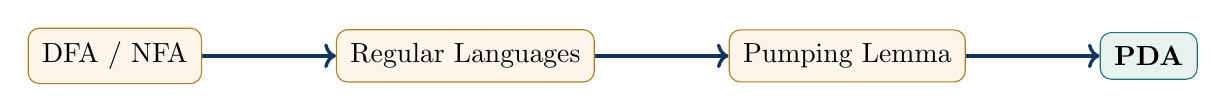
\begin{tikzpicture}[node distance=1.7cm]
    \node[note] (dfa) {DFA / NFA};
    \node[note,right=of dfa] (reg) {Regular Languages};
    \node[note,right=of reg] (pump) {Pumping Lemma};
    \node[note,right=of pump,draw=toccyan,fill=toccyan!10] (pda) {\textbf{PDA}};
    \draw[->,very thick,tocblue] (dfa)--(reg);
    \draw[->,very thick,tocblue] (reg)--(pump);
    \draw[->,very thick,tocblue] (pump)--(pda);
\end{tikzpicture}

\vspace{1.2em}
The Pumping Lemma showed that some languages need more memory than a finite automaton possesses.

\vspace{0.8em}
\begin{alertblock}{Today’s question}
What is the smallest useful extension of a finite automaton that can remember an unbounded amount of structured information?
\end{alertblock}
\end{frame}

% -------------------------------------------------
\begin{frame}{Learning Goals}
By the end of this lecture, you should be able to:

\begin{enumerate}
    \item explain why a stack enables nonregular behavior;
    \item describe a PDA informally and formally;
    \item read and write PDA transition labels;
    \item trace a PDA computation using configurations;
    \item design PDAs for equality and palindrome-style languages;
    \item explain where nondeterminism enters PDA design.
\end{enumerate}
\end{frame}

% -------------------------------------------------
\section{Why a Stack?}

% -------------------------------------------------
\begin{frame}{The First Target Language}
Consider
\[
A=\lang{0^n1^n\mid n\ge 0}.
\]

A recognizer must remember how many $0$s appeared and then verify that exactly the same number of $1$s follows.

\vspace{0.8em}
\begin{columns}[T,onlytextwidth]
\column{0.48\textwidth}
\begin{block}{A DFA has}
\begin{itemize}
    \item finitely many states;
    \item no growing memory;
    \item no way to store arbitrary $n$.
\end{itemize}
\end{block}

\column{0.48\textwidth}
\begin{exampleblock}{A stack can}
\begin{itemize}
    \item push one marker per $0$;
    \item pop one marker per $1$;
    \item detect mismatch or wrong order.
\end{itemize}
\end{exampleblock}
\end{columns}
\end{frame}

% -------------------------------------------------
\begin{frame}{A Stack Is Last-In, First-Out}
\begin{columns}[c,onlytextwidth]
\column{0.50\textwidth}
A stack supports two basic operations:

\begin{itemize}
    \item \textbf{push:} place a symbol on top;
    \item \textbf{pop:} remove the top symbol.
\end{itemize}

\vspace{0.8em}
Only the top symbol is directly accessible.

\column{0.45\textwidth}
\centering
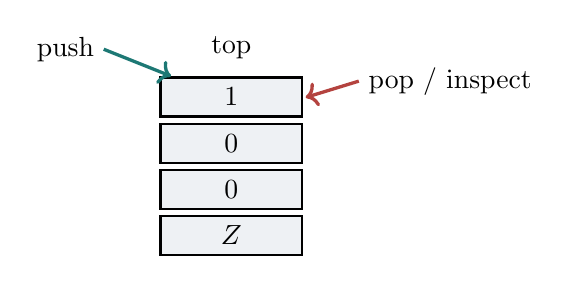
\begin{tikzpicture}[scale=0.9]
    \foreach \y/\s in {0/$Z$,0.65/$0$,1.30/$0$,1.95/$1$}{
        \draw[thick,fill=tocblue!7] (0,\y) rectangle (2,\y+0.55);
        \node at (1,\y+0.275) {\s};
    }
    \node[above] at (1,2.62) {top};
    \draw[->,very thick,tocred] (2.8,2.45)--(2.05,2.22);
    \node[right] at (2.8,2.45) {pop / inspect};
    \draw[->,very thick,toccyan] (-0.8,2.9)--(0.15,2.52);
    \node[left] at (-0.8,2.9) {push};
\end{tikzpicture}
\end{columns}
\end{frame}

% -------------------------------------------------
\begin{frame}{The PDA Architecture}
A \alert{pushdown automaton} is roughly an NFA equipped with a stack.

\vspace{0.8em}
\centering
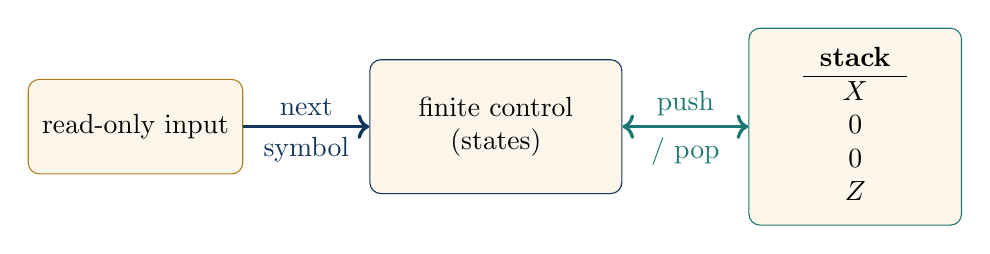
\begin{tikzpicture}[node distance=1.6cm]
    \node[note,minimum width=2.7cm,minimum height=1.2cm] (input) {read-only input};
    \node[note,right=of input,minimum width=3.2cm,minimum height=1.7cm,draw=tocblue,align=center] (control) {finite control\\(states)};
    \node[note,right=of control,minimum width=2.7cm,minimum height=2.5cm,draw=toccyan] (stack) {\begin{tabular}{c}\textbf{stack}\\\hline $X$\\$0$\\$0$\\$Z$\end{tabular}};
    \draw[->,very thick,tocblue] (input)--node[above]{next} node[below]{symbol} (control);
    \draw[<->,very thick,toccyan] (control)--node[above]{push} node[below]{/ pop}(stack);
\end{tikzpicture}

\vspace{0.9em}
At each step, the PDA will use:
\[
\text{current state},\qquad
\text{next input symbol or }\eps,\qquad
\text{top stack symbol or }\eps.
\]
\end{frame}

% -------------------------------------------------
\begin{frame}{Running Strategy for $0^n1^n$}
\begin{enumerate}
    \item While reading $0$s, push one $0$ onto the stack for each input $0$.
    \item When the first $1$ arrives, switch to a popping phase.
    \item For every input $1$, pop one stack $0$.
    \item Accept only when the entire input is consumed and the stack is empty.
\end{enumerate}

\vspace{0.8em}
\begin{exampleblock}{Mental picture}
The stack height records the difference
\[
\#0\text{s read}-\#1\text{s read}.
\]
\end{exampleblock}
\end{frame}

% -------------------------------------------------
\begin{frame}{A Trace on $000111$}
\centering
\renewcommand{\arraystretch}{1.25}
\begin{tabular}{lll}
\toprule
\textbf{Unread input} & \textbf{Stack} & \textbf{Action}\\
\midrule
$000111$ & $\eps$ & start\\
$00111$  & $0$    & read $0$, push $0$\\
$0111$   & $00$   & read $0$, push $0$\\
$111$    & $000$  & read $0$, push $0$\\
$11$     & $00$   & read $1$, pop $0$\\
$1$      & $0$    & read $1$, pop $0$\\
$\eps$   & $\eps$ & read $1$, pop $0$; accept\\
\bottomrule
\end{tabular}

\vspace{0.8em}
The stack is unbounded, so the same strategy works for every $n$.
\end{frame}

% -------------------------------------------------
\begin{frame}{How Bad Strings Fail}
\begin{columns}[T,onlytextwidth]
\column{0.31\textwidth}
\begin{alertblock}{$001$}
Input ends while a $0$ remains on the stack.
\end{alertblock}

\column{0.31\textwidth}
\begin{alertblock}{$011$}
The PDA needs to pop after the stack is already empty.
\end{alertblock}

\column{0.31\textwidth}
\begin{alertblock}{$0101$}
After entering the $1$-phase, a later $0$ has no legal move.
\end{alertblock}
\end{columns}

\vspace{1em}
A PDA rejects when \emph{every possible computation branch} fails to accept.
\end{frame}

% -------------------------------------------------
\section{Formal Definition}

% -------------------------------------------------
\begin{frame}{Formal Definition of a PDA}
A pushdown automaton is a $6$-tuple
\[
P=(Q,\Sigma,\Gamma,\delta,q_0,F),
\]
where:

\begin{itemize}
    \item $Q$ is a finite set of states;
    \item $\Sigma$ is the input alphabet;
    \item $\Gamma$ is the stack alphabet;
    \item $q_0\in Q$ is the start state;
    \item $F\subseteq Q$ is the set of accept states;
    \item $\delta$ is the transition function.
\end{itemize}

\vspace{0.4em}
Following Sipser’s formulation,
\[
\delta:Q\times\Sigma_{\eps}\times\Gamma_{\eps}
\longrightarrow
\Pow\bigl(Q\times\Gamma_{\eps}\bigr),
\]
where $\Sigma_{\eps}=\Sigma\cup\{\eps\}$ and $\Gamma_{\eps}=\Gamma\cup\{\eps\}$.
\end{frame}

% -------------------------------------------------
\begin{frame}{Understanding the Six Components}

\begin{block}{Finite control}
The set \(Q\), the start state \(q_0\), and the accept states \(F\)
describe the finite-state part of the machine, just as in an NFA.
\end{block}

\begin{block}{Input and memory}
\begin{itemize}
    \item \(\Sigma\) contains the symbols that may appear in the input.
    \item \(\Gamma\) contains the symbols that may be stored on the stack.
\end{itemize}
\end{block}

\begin{block}{Rules of computation}
The transition function \(\delta\) tells the PDA:
\begin{enumerate}
    \item which input symbol to read, if any;
    \item which stack symbol to remove, if any;
    \item which state to enter;
    \item which stack symbol to place on top, if any.
\end{enumerate}
\end{block}

\end{frame}

% -------------------------------------------------
\begin{frame}{Why Do We Need a Stack Alphabet?}

\small
The input alphabet and the stack alphabet serve different purposes.
\[
\Sigma=\{\text{symbols appearing in the input}\},
\qquad
\Gamma=\{\text{symbols stored as memory}\}.
\]

\begin{exampleblock}{Example: \(L=\{0^n1^n\mid n\geq 0\}\)}
We may use
\[
\Sigma=\{0,1\},
\qquad
\Gamma=\{0,\$\}.
\]

\begin{itemize}
    \item A \(0\) is pushed for every \(0\) read from the input.
    \item A \(0\) is popped for every \(1\) read from the input.
    \item The symbol \(\$\) may be used to mark the bottom of the stack.
\end{itemize}
\end{exampleblock}

The stack alphabet may contain:

\begin{itemize}
    \item symbols from the input alphabet;
    \item completely different bookkeeping symbols;
    \item a special bottom-of-stack marker.
\end{itemize}

There is no requirement that \(\Sigma\) and \(\Gamma\) be the same.

\end{frame}

% -------------------------------------------------
\begin{frame}{Do We Need a Bottom-of-Stack Symbol?}

\small
A special stack symbol such as
\[
\$,\qquad \bot,\qquad \text{or}\qquad Z_0
\]
is often placed at the bottom of the stack.

\begin{block}{Why is it useful?}
It allows the PDA to detect that all previously stored symbols have
been removed.
\end{block}

For example, the initial move may be
\[
\varepsilon,\varepsilon\to \$.
\]

Later, when the PDA sees \(\$\) again, it knows that the useful part of
the stack is empty.

\[
\boxed{\text{Bottom marker reached}}
\quad\Longrightarrow\quad
\boxed{\text{all matching symbols have been popped}}
\]

\begin{alertblock}{Important}
A bottom marker is a convenient design choice, not a required component
of Sipser's formal definition.
\end{alertblock}

\end{frame}

% -------------------------------------------------
\begin{frame}{Understanding the Transition Function}

\small
Sipser defines
\[
\delta:Q\times\Sigma_{\eps}\times\Gamma_{\eps}
\longrightarrow
\Pow(Q\times\Gamma_{\eps}).
\]

A transition examines three pieces of information:

\[
\delta(
\underbrace{q}_{\text{current state}},
\underbrace{a}_{\text{input action}},
\underbrace{X}_{\text{stack action}}
).
\]

If
\(
(r,Y)\in\delta(q,a,X),
\)
then the PDA may:

\begin{enumerate}
    \item move from state \(q\) to state \(r\);
    \item read \(a\) from the input, unless \(a=\eps\);
    \item pop \(X\) from the stack, unless \(X=\eps\);
    \item push \(Y\) onto the stack, unless \(Y=\eps\).
\end{enumerate}

Thus, \(\eps\) means: \(
\boxed{\text{perform no action on that component}}.
\)

\end{frame}

% -------------------------------------------------
\begin{frame}{Four Common Types of PDA Transitions}

\small
Suppose
\(
(r,Y)\in\delta(q,a,X).
\)

Different choices of \(X\) and \(Y\) produce different stack operations.

\begin{center}
\renewcommand{\arraystretch}{1.35}
\begin{tabular}{c|c|l}
\textbf{Pop} & \textbf{Push} & \textbf{Effect} \\ \hline
\(X\) & \(Y\) & Replace \(X\) by \(Y\) \\[0.1em]
\(X\) & \(\eps\) & Pop \(X\) \\[0.1em]
\(\eps\) & \(Y\) & Push \(Y\) \\[0.1em]
\(\eps\) & \(\eps\) & Leave the stack unchanged
\end{tabular}
\end{center}

For example,
\(
(r,\eps)\in\delta(q,1,0)
\)
means:

\begin{quote}
While in \(q\), read a \(1\), pop a \(0\), and move to \(r\).
\end{quote}

Similarly,
\(
(r,0)\in\delta(q,0,\eps)
\)
means:

\begin{quote}
While in \(q\), read a \(0\), push a \(0\), and move to \(r\).
\end{quote}

\end{frame}

% -------------------------------------------------
\begin{frame}{Why Does \(\delta\) Return a Set?}

\small
The codomain of the transition function is
\(
\Pow(Q\times\Gamma_{\eps}),
\)
the set of all possible transition choices.

For example,
\[
\delta(q,\eps,\eps)
=
\{(q_1,\eps),(q_2,\eps)\}.
\]

The PDA may nondeterministically choose either:
\[
q\longrightarrow q_1
\qquad\text{or}\qquad
q\longrightarrow q_2.
\]

\begin{block}{Why is nondeterminism useful?}
A PDA may need to guess:

\begin{itemize}
    \item where the middle of a palindrome occurs;
    \item which part of the input should be compared;
    \item which strategy or branch will lead to acceptance.
\end{itemize}
\end{block}

The input is accepted if \emph{at least one} possible computation
consumes the entire input and reaches an accept state.

\end{frame}

% -------------------------------------------------
\begin{frame}{Unpacking the Transition Function}
Suppose
\[
(r,c)\in\delta(q,a,b).
\]
This means that the PDA may:

\begin{enumerate}
    \item move from state $q$ to state $r$;
    \item read $a$ from the input, unless $a=\eps$;
    \item pop $b$ from the stack, unless $b=\eps$;
    \item push $c$ onto the stack, unless $c=\eps$.
\end{enumerate}

\begin{alertblock}{Important}
Because $\delta$ returns a \emph{set} of possible moves, a PDA is generally nondeterministic.
\end{alertblock}
\end{frame}

% -------------------------------------------------
\begin{frame}{Transition-Diagram Labels}
We write a transition as
\[
\boxed{\text{input},\ \text{pop}\ \longrightarrow\ \text{push}}.
\]

\vspace{0.5em}
\begin{columns}[T,onlytextwidth]
\column{0.48\textwidth}
\begin{block}{$0,\eps\to 0$}
Read an input $0$ and push a $0$. Nothing is popped.
\end{block}

\begin{block}{$1,0\to\eps$}
Read an input $1$ and pop a $0$. Nothing is pushed.
\end{block}

\column{0.48\textwidth}
\begin{block}{$\eps,\eps\to\$$}
Read no input, pop nothing, and push the bottom marker $\$$.
\end{block}

\begin{block}{$\eps,\$\to\eps$}
Read no input and remove the bottom marker.
\end{block}
\end{columns}
\end{frame}

% -------------------------------------------------
\begin{frame}{The Three Roles of $\eps$}
The symbol $\eps$ may appear in three different positions.

\renewcommand{\arraystretch}{1.35}
\begin{tabular}{>{\bfseries}p{0.22\textwidth}p{0.68\textwidth}}
Input is $\eps$ & Change state or stack without consuming input.\\
Pop symbol is $\eps$ & Do not inspect or remove the current stack top.\\
Push symbol is $\eps$ & Do not place a new symbol on the stack.\\
\end{tabular}

\vspace{0.8em}
\begin{alertblock}{Common confusion}
$\eps$ is an instruction meaning ``do nothing here.'' It is not a literal symbol stored in the input or stack.
\end{alertblock}
\end{frame}

% -------------------------------------------------
\begin{frame}{Configurations}
A configuration records the complete instantaneous situation:
\[
(q,w,s),
\]
where
\begin{itemize}
    \item $q$ is the current state;
    \item $w$ is the unread part of the input;
    \item $s$ is the current stack content, with the top written on the left.
\end{itemize}

\vspace{0.6em}
For example,
\[
(q_{\mathrm{pop}},11,00)
\]
means: the PDA is in the popping state, still has $11$ to read, and has two $0$s on its stack.
\end{frame}

% -------------------------------------------------
\begin{frame}{One Computation Step}
If
\[
(r,c)\in\delta(q,a,b),
\]
then we may write
\[
(q,aw,bs)\turn(r,w,cs).
\]
Here $a\in\Sigma_{\eps}$ and $b,c\in\Gamma_{\eps}$.

\vspace{0.8em}
The notation is interpreted naturally when one of $a,b,c$ equals $\eps$:

\begin{itemize}
    \item $a=\eps$: no input symbol disappears;
    \item $b=\eps$: no stack symbol disappears;
    \item $c=\eps$: no stack symbol is added.
\end{itemize}
\end{frame}

% -------------------------------------------------
\begin{frame}{Acceptance by Final State}
A PDA $P$ accepts input $w$ if there is a sequence of legal moves such that
\[
(q_0,w,\eps)\turns(q_f,\eps,s)
\]
for some $q_f\in F$ and some stack content $s\in\Gamma^{*}$.

\vspace{0.8em}
\begin{exampleblock}{Two requirements}
\begin{enumerate}
    \item The entire input must be consumed.
    \item At least one computation branch must finish in an accept state.
\end{enumerate}
\end{exampleblock}

\vspace{0.4em}
Acceptance by empty stack is another standard convention; it recognizes the same class of languages. We will see that later in the course.
\end{frame}

% -------------------------------------------------
\section{A Complete PDA}

% -------------------------------------------------
\begin{frame}{PDA for $A=\{0^n1^n\mid n\ge 0\}$}
\centering
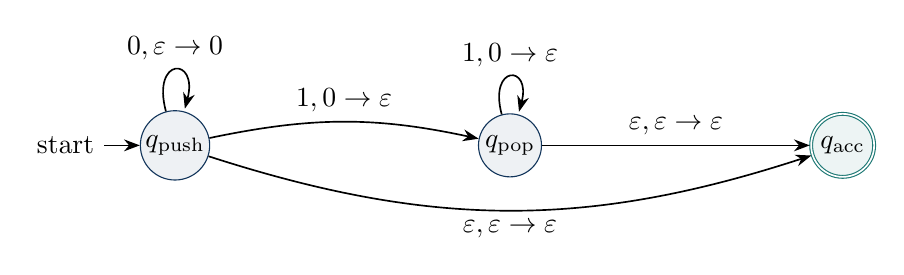
\begin{tikzpicture}[node distance=3.4cm,auto]
    \node[pda,initial] (push) {$q_{\mathrm{push}}$};
    \node[pda,right=of push] (pop) {$q_{\mathrm{pop}}$};
    \node[accept,right=of pop] (acc) {$q_{\mathrm{acc}}$};

    \path
    (push) edge[loop above] node {$0,\eps\to 0$} (push)
    (push) edge[bend left=12] node {$1,0\to\eps$} (pop)
    (push) edge[bend right=18] node[below] {$\eps,\eps\to\eps$} (acc)
    (pop) edge[loop above] node {$1,0\to\eps$} (pop)
    (pop) edge node {$\eps,\eps\to\eps$} (acc);
\end{tikzpicture}

\vspace{1em}
The direct $q_{\mathrm{push}}\to q_{\mathrm{acc}}$ transition handles $n=0$, i.e., the empty string.
\end{frame}

% -------------------------------------------------
\begin{frame}{Why This PDA Is Correct}
A correctness argument has two directions.

\begin{block}{Every string in $A$ is accepted}
For $0^n1^n$, the PDA pushes exactly $n$ markers, then pops exactly $n$ markers, consumes the input, and reaches $q_{\mathrm{acc}}$.
\end{block}

\begin{alertblock}{Every accepted string belongs to $A$}
An accepting computation must first read only $0$s while pushing, then read only $1$s while popping. Each $1$ consumes exactly one earlier $0$ marker, so the two counts are equal.
\end{alertblock}
\end{frame}

% -------------------------------------------------
\begin{frame}{Formal Trace of $0011$}
Using configurations:
\begin{align*}
(q_{\mathrm{push}},0011,\eps)
&\turn(q_{\mathrm{push}},011,0)\\
&\turn(q_{\mathrm{push}},11,00)\\
&\turn(q_{\mathrm{pop}},1,0)\\
&\turn(q_{\mathrm{pop}},\eps,\eps)\\
&\turn(q_{\mathrm{acc}},\eps,\eps).
\end{align*}

\vspace{0.6em}
\begin{exampleblock}{Check yourself}
At which step does the machine commit to the second phase?
\end{exampleblock}
\end{frame}

% -------------------------------------------------
\section{Why Nondeterminism Matters}

% -------------------------------------------------
\begin{frame}{A New Language: Even Palindromes}
Consider
\[
B=\lang{ww^R\mid w\in\{0,1\}^{*}}.
\]
Examples include
\[
\eps,\quad 00,\quad 11,\quad 0110,\quad 1001,\quad 010010.
\]

A natural plan is:
\begin{enumerate}
    \item push symbols from the first half;
    \item at the midpoint, switch modes;
    \item compare the second half against the stack.
\end{enumerate}

\begin{alertblock}{The difficulty}
There is no delimiter telling us where the midpoint occurs.
\end{alertblock}
\end{frame}

% -------------------------------------------------
\begin{frame}{Guess the Midpoint}
A nondeterministic PDA can branch at every position:

\begin{itemize}
    \item one branch keeps pushing;
    \item another branch guesses, ``the first half ends here,'' and begins popping.
\end{itemize}

\vspace{0.8em}
\begin{exampleblock}{Acceptance semantics}
The input is accepted if \emph{one} branch guesses the correct midpoint and all symbol comparisons succeed.
\end{exampleblock}

\vspace{0.6em}
A wrong guess is harmless: that branch simply gets stuck or rejects.
\end{frame}

% -------------------------------------------------
\begin{frame}{PDA for $B=\{ww^R\}$}
\centering
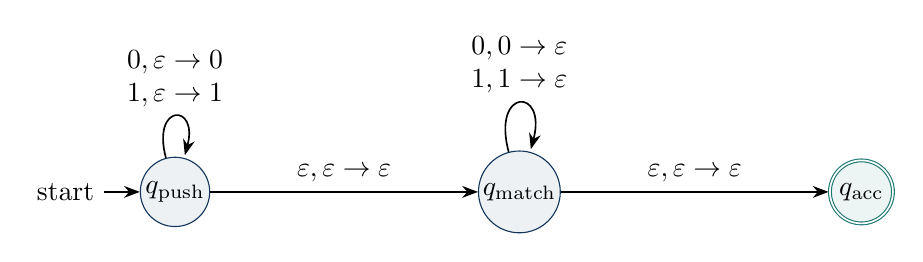
\begin{tikzpicture}[node distance=3.4cm,auto]
    \node[pda,initial] (push) {$q_{\mathrm{push}}$};
    \node[pda,right=of push] (match) {$q_{\mathrm{match}}$};
    \node[accept,right=of match] (acc) {$q_{\mathrm{acc}}$};

    \path
    (push) edge[loop above] node[align=center] {$0,\eps\to0$\\$1,\eps\to1$} (push)
    (push) edge node {$\eps,\eps\to\eps$} (match)
    (match) edge[loop above] node[align=center] {$0,0\to\eps$\\$1,1\to\eps$} (match)
    (match) edge node {$\eps,\eps\to\eps$} (acc);
\end{tikzpicture}

\vspace{0.8em}
The $\eps$-move guesses the midpoint. The matching phase verifies the reverse order.
\end{frame}

% -------------------------------------------------
\begin{frame}{One Accepting Branch for $0110$}
\begin{align*}
(q_{\mathrm{push}},0110,\eps)
&\turn(q_{\mathrm{push}},110,0)\\
&\turn(q_{\mathrm{push}},10,10)\\
&\turn(q_{\mathrm{match}},10,10)\qquad\text{(guess midpoint)}\\
&\turn(q_{\mathrm{match}},0,0)\\
&\turn(q_{\mathrm{match}},\eps,\eps)\\
&\turn(q_{\mathrm{acc}},\eps,\eps).
\end{align*}

Other branches may guess too early or too late; they reject.
\end{frame}

% -------------------------------------------------
\begin{frame}{A Delimiter Removes the Guess}
For
\[
C=\lang{w\#w^R\mid w\in\{0,1\}^{*}},
\]
the symbol $\#$ explicitly marks the midpoint.

\vspace{0.8em}
\begin{columns}[T,onlytextwidth]
\column{0.48\textwidth}
\begin{block}{Before $\#$}
Push every $0$ or $1$.
\end{block}

\column{0.48\textwidth}
\begin{exampleblock}{After $\#$}
Pop and compare every symbol.
\end{exampleblock}
\end{columns}

\vspace{0.8em}
This language can be recognized without guessing the boundary; it illustrates the difference between deterministic and nondeterministic behavior.
\end{frame}

% -------------------------------------------------
\begin{frame}{Another Example}
Consider
\[
D=\lang{0^i1^j2^k\mid i=j\text{ or }j=k}.
\]

A PDA can nondeterministically choose one of two jobs:

\begin{enumerate}
    \item verify $i=j$ and ignore the number of $2$s;
    \item ignore the number of $0$s and verify $j=k$.
\end{enumerate}

\vspace{0.8em}
\begin{exampleblock}{Key principle}
Nondeterministic branching naturally implements a union:
\[
L_1\cup L_2.
\]
\end{exampleblock}
\end{frame}

% -------------------------------------------------
\section{Designing PDAs}

% -------------------------------------------------
\begin{frame}{PDA Design Pattern 1: Count and Match}
Use the stack as an unbounded counter when the later input must match an earlier quantity.

\[
\underbrace{0\cdots0}_{\text{push}}
\underbrace{1\cdots1}_{\text{pop}}
\]

Typical languages:
\[
\lang{a^nb^n\mid n\ge0},
\qquad
\lang{a^ib^jc^k\mid i=j}.
\]

\begin{alertblock}{Caution}
The stack is not a random-access counter. Its LIFO order becomes important when symbols, not just counts, must be compared.
\end{alertblock}
\end{frame}

% -------------------------------------------------
\begin{frame}{PDA Design Pattern 2: Store and Reverse}
A stack is ideal when the second part of the input must reproduce the first part in reverse order.

\[
\underbrace{w}_{\text{push symbols}}
\underbrace{w^R}_{\text{pop and compare}}
\]

Typical languages:
\[
\lang{w\#w^R},
\qquad
\lang{ww^R}.
\]

The LIFO rule automatically reverses the stored sequence.
\end{frame}

% -------------------------------------------------
\begin{frame}{PDA Design Pattern 3: Guess a Boundary}
When a phase change is not marked in the input:

\begin{enumerate}
    \item create an $\eps$-transition to a new phase;
    \item allow the machine to take it at any point;
    \item ensure only the correct guess can complete an accepting computation.
\end{enumerate}

\vspace{0.8em}
Common uses:
\begin{itemize}
    \item guessing a midpoint;
    \item guessing which condition of a union will hold;
    \item guessing a decomposition of the input.
\end{itemize}
\end{frame}

% -------------------------------------------------
\begin{frame}{A Practical Design Checklist}
When constructing a PDA, ask:

\begin{enumerate}
    \item What information must survive for an unbounded distance?
    \item What exactly should each stack symbol mean?
    \item When does the machine push, and when does it pop?
    \item Is the phase boundary visible or must it be guessed?
    \item What malformed input orders should have no transition?
    \item How are $\eps$ and the empty input handled?
    \item Why can no string outside the language reach an accept state?
\end{enumerate}
\end{frame}

% -------------------------------------------------
\begin{frame}{Common Mistakes}
\begin{enumerate}
    \item Accepting as soon as the stack becomes empty, even though unread input remains.
    \item Forgetting the empty string when $n=0$ is allowed.
    \item Popping a symbol without checking whether it matches.
    \item Using a transition that accidentally permits symbols in the wrong order.
    \item Treating nondeterminism as ``try one arbitrary choice'' rather than ``accept if some branch succeeds.''
    \item Confusing $\eps$ with a real input or stack symbol.
\end{enumerate}
\end{frame}

% -------------------------------------------------
\begin{frame}{DFA Versus PDA}
\centering
\renewcommand{\arraystretch}{1.35}
\begin{tabular}{p{0.25\textwidth}p{0.30\textwidth}p{0.34\textwidth}}
\toprule
& \textbf{Finite Automaton} & \textbf{Pushdown Automaton}\\
\midrule
Memory & current state only & state plus unbounded stack\\
Access & finite control & top of stack only\\
Typical power & local patterns & nested / matched structure\\
Example & strings ending in $01$ & $0^n1^n$, palindromes\\
Nondeterminism & no extra language power & strictly increases power over deterministic PDAs\\
\bottomrule
\end{tabular}
\end{frame}

% -------------------------------------------------
\begin{frame}{What One Stack Still Cannot Do}
A PDA is more powerful than a finite automaton, but it is not all-powerful.

\vspace{0.8em}
The language
\[
E=\lang{0^n1^n2^n\mid n\ge0}
\]
cannot be recognized by any one-stack PDA.

\vspace{0.8em}
\begin{alertblock}{Intuition, not yet a proof}
After using the stack to compare the $0$s with the $1$s, the machine no longer has enough independent information to compare the same $n$ with the $2$s.
\end{alertblock}

A formal impossibility proof will come later.
\end{frame}

% -------------------------------------------------

% =================================================
\section{Ten Worked-Out PDA Examples}
% =================================================

% -------------------------------------------------
\begin{frame}{How to Read the Worked Examples}
\small
In all examples below, the transition label has the same meaning as before:
\[
\boxed{\text{input},\ \text{pop}\ \to\ \text{push}}.
\]

We use a bottom-of-stack marker \(Z\).  Each PDA accepts by final state, but the only accepting move is made after \(Z\) becomes visible again.

\begin{exampleblock}{Design pattern}
\begin{enumerate}
    \item Push symbols while reading the part whose size or content must be remembered.
    \item Pop symbols while reading the part that must match it.
    \item Let wrong order, wrong symbol, or wrong count get stuck automatically.
\end{enumerate}
\end{exampleblock}
\end{frame}

% -------------------------------------------------
\begin{frame}{Example 1: \(L_1=\{a^n b^{2n}\mid n\ge 0\}\)}
\small
\begin{columns}[T,onlytextwidth]
\column{0.39\textwidth}
\begin{block}{Idea}
Push one \(X\) for each \(a\).  Then read the \(b\)'s in pairs.  The second \(b\) of every pair pops one \(X\).
\end{block}

\begin{alertblock}{Failure modes}
Odd number of \(b\)'s, too few \(b\)'s, too many \(b\)'s, or an \(a\) after a \(b\) gets stuck.
\end{alertblock}

\column{0.58\textwidth}
\centering
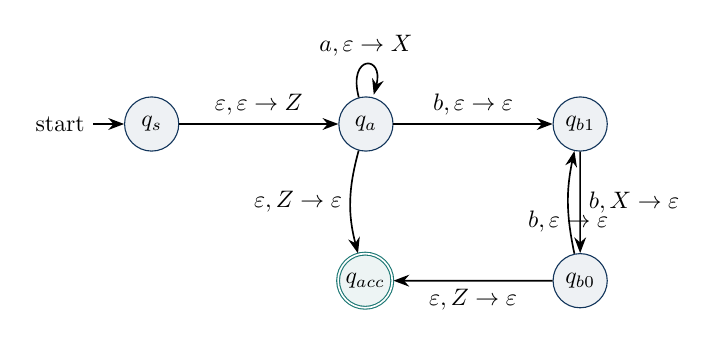
\begin{tikzpicture}[node distance=2.35cm,auto,scale=0.86,transform shape]
    \node[pda,initial] (s) {$q_s$};
    \node[pda,right=of s] (a) {$q_a$};
    \node[pda,right=of a] (odd) {$q_{b1}$};
    \node[pda,below=1.5cm of odd] (even) {$q_{b0}$};
    \node[accept,left=2.35cm of even] (acc) {$q_{acc}$};

    \path
    (s) edge node {$\eps,\eps\to Z$} (a)
    (a) edge[loop above] node {$a,\eps\to X$} (a)
    (a) edge node {$b,\eps\to\eps$} (odd)
    (odd) edge node[right] {$b,X\to\eps$} (even)
    (even) edge[bend left=12] node[below] {$b,\eps\to\eps$} (odd)
    (a) edge[bend right=15] node[left] {$\eps,Z\to\eps$} (acc)
    (even) edge node[below] {$\eps,Z\to\eps$} (acc);
\end{tikzpicture}
\end{columns}
\end{frame}

% -------------------------------------------------
\begin{frame}{Example 1 Worked Trace}
\small
For input \(aabbbb\):
\[
(q_a,aabbbb,Z)
\turn(q_a,abbbb,XZ)
\turn(q_a,bbbb,XXZ)
\turn(q_{b1},bbb,XXZ)
\turn(q_{b0},bb,XZ)
\turn(q_{b1},b,XZ)
\turn(q_{b0},\eps,Z)
\turn(q_{acc},\eps,\eps).
\]

\begin{exampleblock}{Correctness}
After \(n\) copies of \(a\), the stack contains \(X^nZ\).  Exactly two \(b\)'s are needed to remove one \(X\).  Acceptance is possible exactly when all input is consumed and all \(X\)'s are removed.
\end{exampleblock}
\end{frame}

% -------------------------------------------------
\begin{frame}{Example 2: \(L_2=\{a^i b^j\mid i\le j\}\)}
\small
\begin{columns}[T,onlytextwidth]
\column{0.36\textwidth}
\begin{block}{Idea}
Push one \(X\) for each \(a\).  Each early \(b\) cancels one \(a\).  After the stack returns to \(Z\), extra \(b\)'s are harmless.
\end{block}

\column{0.61\textwidth}
\centering
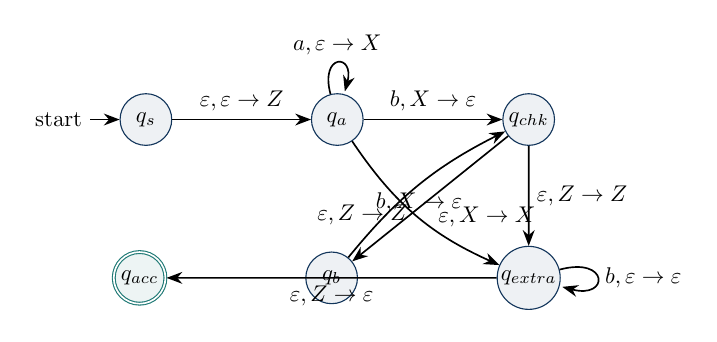
\begin{tikzpicture}[node distance=2.15cm,auto,scale=0.82,transform shape]
    \node[pda,initial] (s) {$q_s$};
    \node[pda,right=of s] (a) {$q_a$};
    \node[pda,right=of a] (chk) {$q_{chk}$};
    \node[pda,below=1.55cm of chk] (more) {$q_{extra}$};
    \node[pda,left=of more] (b) {$q_b$};
    \node[accept,left=of b] (acc) {$q_{acc}$};

    \path
    (s) edge node {$\eps,\eps\to Z$} (a)
    (a) edge[loop above] node {$a,\eps\to X$} (a)
    (a) edge node {$b,X\to\eps$} (chk)
    (chk) edge node {$\eps,X\to X$} (b)
    (chk) edge node[right] {$\eps,Z\to Z$} (more)
    (b) edge[bend left=12] node[below] {$b,X\to\eps$} (chk)
    (a) edge[bend right=16] node[left] {$\eps,Z\to Z$} (more)
    (more) edge[loop right] node {$b,\eps\to\eps$} (more)
    (more) edge node[below] {$\eps,Z\to\eps$} (acc);
\end{tikzpicture}
\end{columns}
\end{frame}

% -------------------------------------------------
\begin{frame}{Example 2 Worked Trace}
\small
For input \(aabbb\):
\[
(q_a,aabbb,Z)
\turn(q_a,abbb,XZ)
\turn(q_a,bbb,XXZ)
\turn(q_{chk},bb,XZ)
\turn(q_b,bb,XZ)
\turn(q_{chk},b,Z)
\turn(q_{extra},b,Z)
\turn(q_{extra},\eps,Z)
\turn(q_{acc},\eps,\eps).
\]

\begin{alertblock}{Why \(aa b\) rejects}
Only one \(b\) is available, so only one \(X\) can be removed.  The stack still contains an unmatched \(X\), so the accepting transition on \(Z\) is impossible.
\end{alertblock}
\end{frame}

% -------------------------------------------------
\begin{frame}{Example 3: \(L_3=\{a^i b^j c^k\mid i=k\}\)}
\small
\begin{columns}[T,onlytextwidth]
\column{0.37\textwidth}
\begin{block}{Idea}
Only the number of \(a\)'s and \(c\)'s matters. Push for \(a\)'s, ignore the middle \(b\)'s, and pop for \(c\)'s.
\end{block}

\column{0.60\textwidth}
\centering
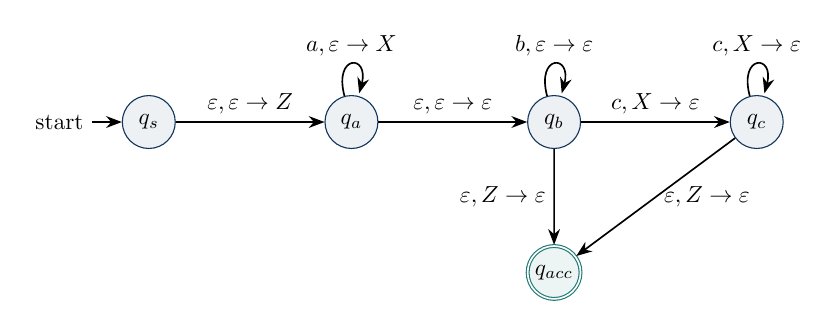
\begin{tikzpicture}[node distance=2.25cm,auto,scale=0.84,transform shape]
    \node[pda,initial] (s) {$q_s$};
    \node[pda,right=of s] (a) {$q_a$};
    \node[pda,right=of a] (b) {$q_b$};
    \node[pda,right=of b] (c) {$q_c$};
    \node[accept,below=1.45cm of b] (acc) {$q_{acc}$};

    \path
    (s) edge node {$\eps,\eps\to Z$} (a)
    (a) edge[loop above] node {$a,\eps\to X$} (a)
    (a) edge node {$\eps,\eps\to\eps$} (b)
    (b) edge[loop above] node {$b,\eps\to\eps$} (b)
    (b) edge node {$c,X\to\eps$} (c)
    (c) edge[loop above] node {$c,X\to\eps$} (c)
    (b) edge node[left] {$\eps,Z\to\eps$} (acc)
    (c) edge node[right] {$\eps,Z\to\eps$} (acc);
\end{tikzpicture}
\end{columns}

\vspace{0.6em}
The \(\eps\)-move from \(q_a\) to \(q_b\) guesses that the block of \(a\)'s has ended.
\end{frame}

% -------------------------------------------------
\begin{frame}{Example 3 Worked Trace}
\small
For input \(aabbcc\):
\[
(q_a,aabbcc,Z)
\turn(q_a,abbcc,XZ)
\turn(q_a,bbcc,XXZ)
\turn(q_b,bbcc,XXZ)
\turn(q_b,bcc,XXZ)
\turn(q_b,cc,XXZ)
\turn(q_c,c,XZ)
\turn(q_c,\eps,Z)
\turn(q_{acc},\eps,\eps).
\]

\begin{exampleblock}{Correctness}
The \(b\)'s never change the stack.  Therefore the stack height records exactly \(i-k\).  Acceptance occurs exactly when this difference returns to zero after the input is consumed.
\end{exampleblock}
\end{frame}

% -------------------------------------------------
\begin{frame}{Example 4: \(L_4=\{w\#w^R\mid w\in\{0,1\}^*\}\)}
\small
\begin{columns}[T,onlytextwidth]
\column{0.36\textwidth}
\begin{block}{Idea}
Before \(\#\), push each symbol.  After \(\#\), pop and compare.  The stack reverses the first half automatically.
\end{block}

\column{0.61\textwidth}
\centering
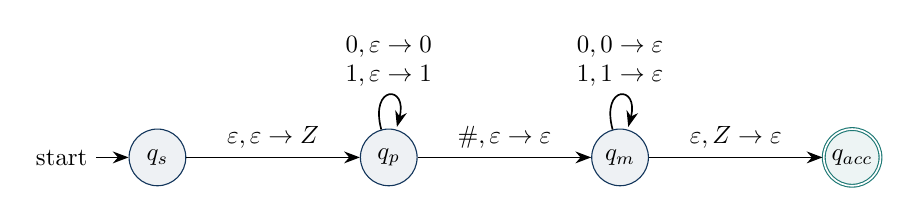
\begin{tikzpicture}[node distance=2.45cm,auto,scale=0.9,transform shape]
    \node[pda,initial] (s) {$q_s$};
    \node[pda,right=of s] (push) {$q_p$};
    \node[pda,right=of push] (match) {$q_m$};
    \node[accept,right=of match] (acc) {$q_{acc}$};

    \path
    (s) edge node {$\eps,\eps\to Z$} (push)
    (push) edge[loop above] node[align=center] {$0,\eps\to0$\\$1,\eps\to1$} (push)
    (push) edge node {$\#,\eps\to\eps$} (match)
    (match) edge[loop above] node[align=center] {$0,0\to\eps$\\$1,1\to\eps$} (match)
    (match) edge node {$\eps,Z\to\eps$} (acc);
\end{tikzpicture}
\end{columns}
\end{frame}

% -------------------------------------------------
\begin{frame}{Example 4 Worked Trace}
\small
For input \(01\#10\):
\[
(q_p,01\#10,Z)
\turn(q_p,1\#10,0Z)
\turn(q_p,\#10,10Z)
\turn(q_m,10,10Z)
\turn(q_m,0,0Z)
\turn(q_m,\eps,Z)
\turn(q_{acc},\eps,\eps).
\]

\begin{alertblock}{Why \(01\#01\) rejects}
After \(\#\), the first symbol is \(0\), but the stack top is \(1\).  There is no transition \(0,1\to\eps\), so the computation gets stuck.
\end{alertblock}
\end{frame}

% -------------------------------------------------
\begin{frame}{Example 5: \(L_5=\{w\in\{0,1\}^*\mid w=w^R\}\)}
\small
\begin{columns}[T,onlytextwidth]
\column{0.37\textwidth}
\begin{block}{Idea}
Push a prefix, nondeterministically guess the middle, and then pop to match the suffix.
\end{block}

\begin{exampleblock}{Two guesses}
\begin{itemize}
    \item \(\eps\)-move: even length.
    \item Consume one symbol: odd length.
\end{itemize}
\end{exampleblock}

\column{0.60\textwidth}
\centering
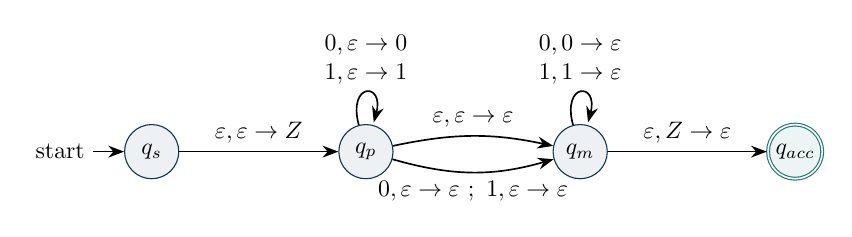
\begin{tikzpicture}[node distance=2.35cm,auto,scale=0.86,transform shape]
    \node[pda,initial] (s) {$q_s$};
    \node[pda,right=of s] (push) {$q_p$};
    \node[pda,right=of push] (match) {$q_m$};
    \node[accept,right=of match] (acc) {$q_{acc}$};

    \path
    (s) edge node {$\eps,\eps\to Z$} (push)
    (push) edge[loop above] node[align=center] {$0,\eps\to0$\\$1,\eps\to1$} (push)
    (push) edge[bend left=12] node[above] {$\eps,\eps\to\eps$} (match)
    (push) edge[bend right=16] node[below] {$0,\eps\to\eps\ ;\ 1,\eps\to\eps$} (match)
    (match) edge[loop above] node[align=center] {$0,0\to\eps$\\$1,1\to\eps$} (match)
    (match) edge node {$\eps,Z\to\eps$} (acc);
\end{tikzpicture}
\end{columns}
\end{frame}

% -------------------------------------------------
\begin{frame}{Example 5 Worked Trace}
\small
One accepting branch for \(01010\):
\[
(q_p,01010,Z)
\turn(q_p,1010,0Z)
\turn(q_p,010,10Z)
\turn(q_m,10,10Z) \quad\text{skip the middle }0
\turn(q_m,0,0Z)
\turn(q_m,\eps,Z)
\turn(q_{acc},\eps,\eps).
\]

\begin{alertblock}{Role of nondeterminism}
Wrong midpoint guesses may fail.  That is fine: the string is accepted because one branch guesses the correct middle.
\end{alertblock}
\end{frame}

% -------------------------------------------------
\begin{frame}{Example 6: Balanced Parentheses}
\small
\[
L_6=\{w\in\{\mathtt{(},\mathtt{)}\}^*\mid w\text{ is balanced}\}.
\]

\begin{columns}[T,onlytextwidth]
\column{0.38\textwidth}
\begin{block}{Idea}
Push one \(X\) for every opening parenthesis.  Pop one \(X\) for every closing parenthesis.
\end{block}

\column{0.59\textwidth}
\centering
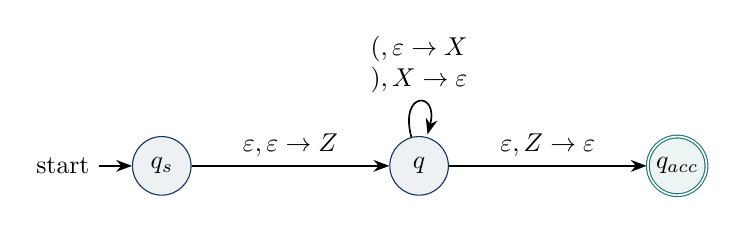
\begin{tikzpicture}[node distance=2.7cm,auto,scale=0.93,transform shape]
    \node[pda,initial] (s) {$q_s$};
    \node[pda,right=of s] (q) {$q$};
    \node[accept,right=of q] (acc) {$q_{acc}$};

    \path
    (s) edge node {$\eps,\eps\to Z$} (q)
    (q) edge[loop above] node[align=center] {$\mathtt{(},\eps\to X$\\$\mathtt{)},X\to\eps$} (q)
    (q) edge node {$\eps,Z\to\eps$} (acc);
\end{tikzpicture}
\end{columns}

\vspace{0.4em}
A prefix with more closing than opening parentheses gets stuck because there is no \(X\) to pop.
\end{frame}

% -------------------------------------------------
\begin{frame}{Example 6 Worked Trace}
\small
For input \(\mathtt{(()())}\):
\[
(q,\mathtt{(()())},Z)
\turn(q,\mathtt{()())},XZ)
\turn(q,\mathtt{)())},XXZ)
\turn(q,\mathtt{())},XZ)
\turn(q,\mathtt{))},XXZ)
\turn(q,\mathtt{)},XZ)
\turn(q,\eps,Z)
\turn(q_{acc},\eps,\eps).
\]

\begin{exampleblock}{Invariant}
At every moment, the stack contains exactly the unmatched opening parentheses of the prefix already read.
\end{exampleblock}
\end{frame}

% -------------------------------------------------
\begin{frame}{Example 7: \(L_7=\{w\in\{0,1\}^*\mid \#_0(w)=\#_1(w)\}\)}
\small
\begin{block}{Idea}
The stack stores the current imbalance.  In state \(q_0\), \(X\)'s mean extra \(0\)'s.  In state \(q_1\), \(X\)'s mean extra \(1\)'s.  Reading the opposite symbol cancels one \(X\).
\end{block}

\centering
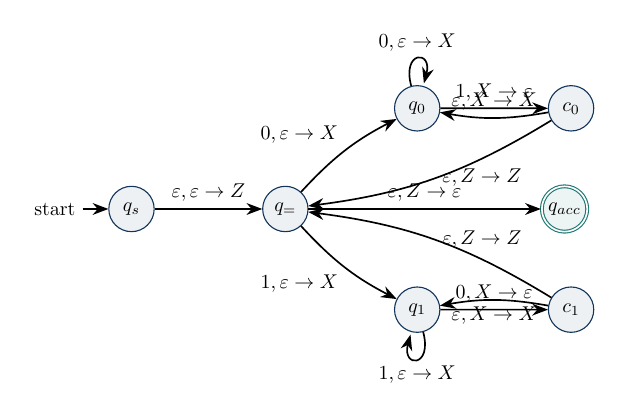
\begin{tikzpicture}[node distance=1.9cm,auto,scale=0.72,transform shape]
    \node[pda,initial] (s) {$q_s$};
    \node[pda,right=of s] (eq) {$q_=$};
    \node[pda,above right=1.2cm and 1.75cm of eq] (z) {$q_0$};
    \node[pda,right=of z] (cz) {$c_0$};
    \node[pda,below right=1.2cm and 1.75cm of eq] (o) {$q_1$};
    \node[pda,right=of o] (co) {$c_1$};
    \node[accept,right=4.1cm of eq] (acc) {$q_{acc}$};

    \path
    (s) edge node {$\eps,\eps\to Z$} (eq)
    (eq) edge[bend left=10] node[above left] {$0,\eps\to X$} (z)
    (eq) edge[bend right=10] node[below left] {$1,\eps\to X$} (o)
    (eq) edge node {$\eps,Z\to\eps$} (acc)
    (z) edge[loop above] node {$0,\eps\to X$} (z)
    (z) edge node {$1,X\to\eps$} (cz)
    (cz) edge[bend left=10] node[above] {$\eps,X\to X$} (z)
    (cz) edge[bend left=12] node[right] {$\eps,Z\to Z$} (eq)
    (o) edge[loop below] node {$1,\eps\to X$} (o)
    (o) edge node {$0,X\to\eps$} (co)
    (co) edge[bend right=10] node[below] {$\eps,X\to X$} (o)
    (co) edge[bend right=12] node[right] {$\eps,Z\to Z$} (eq);
\end{tikzpicture}
\end{frame}

% -------------------------------------------------
\begin{frame}{Example 7 Worked Trace}
\small
For input \(001011\):
\[
\begin{aligned}
(q_=,001011,Z)
&\turn(q_0,01011,XZ)
\turn(q_0,1011,XXZ)
\turn(c_0,011,XZ)\turn(q_0,011,XZ)\\
&\turn(q_0,11,XXZ)
\turn(c_0,1,XZ)\turn(q_0,1,XZ)
\turn(c_0,\eps,Z)\turn(q_=,\eps,Z)
\turn(q_{acc},\eps,\eps).
\end{aligned}
\]

\begin{exampleblock}{Correctness}
The machine never stores both kinds of excess at once.  It either stores unmatched \(0\)'s, unmatched \(1\)'s, or nothing beyond \(Z\).  Thus acceptance at \(q_=\) means the two counts are equal.
\end{exampleblock}
\end{frame}

% -------------------------------------------------
\begin{frame}{Example 8: \(L_8=\{a^i b^j c^k\mid i=j\text{ or }j=k\}\)}
\small
\begin{block}{Idea}
Use nondeterminism to choose which equality to verify.  One branch checks \(i=j\) and ignores \(c\)'s.  The other branch ignores \(a\)'s and checks \(j=k\).
\end{block}

\centering
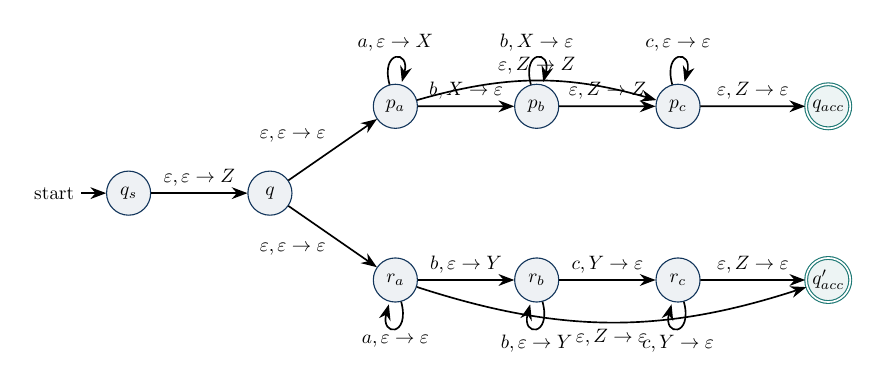
\begin{tikzpicture}[node distance=1.75cm,auto,scale=0.70,transform shape]
    \node[pda,initial] (s) {$q_s$};
    \node[pda,right=of s] (q) {$q$};
    \node[pda,above right=1.0cm and 1.7cm of q] (pa) {$p_a$};
    \node[pda,right=of pa] (pb) {$p_b$};
    \node[pda,right=of pb] (pc) {$p_c$};
    \node[pda,below right=1.0cm and 1.7cm of q] (ra) {$r_a$};
    \node[pda,right=of ra] (rb) {$r_b$};
    \node[pda,right=of rb] (rc) {$r_c$};
    \node[accept,right=1.9cm of pc] (acc1) {$q_{acc}$};
    \node[accept,right=1.9cm of rc] (acc2) {$q'_{acc}$};

    \path
    (s) edge node {$\eps,\eps\to Z$} (q)
    (q) edge node[above left] {$\eps,\eps\to\eps$} (pa)
    (q) edge node[below left] {$\eps,\eps\to\eps$} (ra)
    (pa) edge[loop above] node {$a,\eps\to X$} (pa)
    (pa) edge node {$b,X\to\eps$} (pb)
    (pb) edge[loop above] node {$b,X\to\eps$} (pb)
    (pb) edge node {$\eps,Z\to Z$} (pc)
    (pa) edge[bend left=16] node[above] {$\eps,Z\to Z$} (pc)
    (pc) edge[loop above] node {$c,\eps\to\eps$} (pc)
    (pc) edge node {$\eps,Z\to\eps$} (acc1)
    (ra) edge[loop below] node {$a,\eps\to\eps$} (ra)
    (ra) edge node {$b,\eps\to Y$} (rb)
    (rb) edge[loop below] node {$b,\eps\to Y$} (rb)
    (rb) edge node {$c,Y\to\eps$} (rc)
    (rc) edge[loop below] node {$c,Y\to\eps$} (rc)
    (ra) edge[bend right=18] node[below] {$\eps,Z\to\eps$} (acc2)
    (rc) edge node {$\eps,Z\to\eps$} (acc2);
\end{tikzpicture}
\end{frame}

% -------------------------------------------------
\begin{frame}{Example 8 Worked Explanation}
\small
For \(a^3b^3c^5\), the upper branch accepts because it verifies \(i=j=3\) and then ignores the five \(c\)'s.

For \(a^4b^2c^2\), the lower branch accepts because it ignores the four \(a\)'s and verifies \(j=k=2\).

\begin{alertblock}{Why nondeterminism is natural here}
The PDA does not need to know in advance which equality is true.  It branches.  If at least one branch verifies its equality and consumes the input, the string is accepted.
\end{alertblock}
\end{frame}

% -------------------------------------------------
\begin{frame}{Example 9: \(L_9=\{a^n b^m c^m d^n\mid m,n\ge0\}\)}
\small
\begin{columns}[T,onlytextwidth]
\column{0.36\textwidth}
\begin{block}{Idea}
This is a nested dependency.  Push \(A\)'s for \(a\)'s, then push \(B\)'s for \(b\)'s.  Pop \(B\)'s on \(c\)'s, then pop \(A\)'s on \(d\)'s.
\end{block}

\column{0.61\textwidth}
\centering
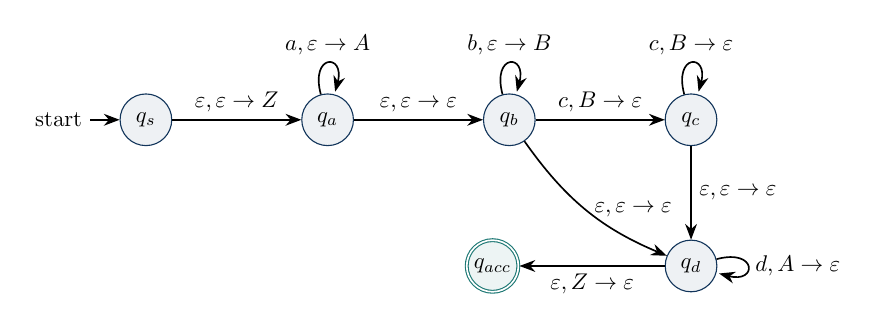
\begin{tikzpicture}[node distance=2.0cm,auto,scale=0.82,transform shape]
    \node[pda,initial] (s) {$q_s$};
    \node[pda,right=of s] (a) {$q_a$};
    \node[pda,right=of a] (b) {$q_b$};
    \node[pda,right=of b] (c) {$q_c$};
    \node[pda,below=1.45cm of c] (d) {$q_d$};
    \node[accept,left=2.25cm of d] (acc) {$q_{acc}$};

    \path
    (s) edge node {$\eps,\eps\to Z$} (a)
    (a) edge[loop above] node {$a,\eps\to A$} (a)
    (a) edge node {$\eps,\eps\to\eps$} (b)
    (b) edge[loop above] node {$b,\eps\to B$} (b)
    (b) edge node {$c,B\to\eps$} (c)
    (c) edge[loop above] node {$c,B\to\eps$} (c)
    (b) edge[bend right=16] node[right] {$\eps,\eps\to\eps$} (d)
    (c) edge node[right] {$\eps,\eps\to\eps$} (d)
    (d) edge[loop right] node {$d,A\to\eps$} (d)
    (d) edge node[below] {$\eps,Z\to\eps$} (acc);
\end{tikzpicture}
\end{columns}
\end{frame}

% -------------------------------------------------
\begin{frame}{Example 9 Worked Trace}
\small
For input \(aabbccdd\):
\[
\begin{aligned}
(q_a,aabbccdd,Z)&\turn(q_a,abbccdd,AZ)\turn(q_a,bbccdd,AAZ)\turn(q_b,bbccdd,AAZ)\\
&\turn(q_b,bccdd,BAAZ)\turn(q_b,ccdd,BBAAZ)\turn(q_c,cdd,BAAZ)\\
&\turn(q_c,dd,AAZ)\turn(q_d,dd,AAZ)\turn(q_d,d,AZ)\turn(q_d,\eps,Z)\turn(q_{acc},\eps,\eps).
\end{aligned}
\]

\begin{exampleblock}{Why LIFO matters}
The \(B\)'s are placed above the \(A\)'s.  Therefore all \(c\)'s must match the \(b\)'s before any \(d\) can match an \(a\).
\end{exampleblock}
\end{frame}

% -------------------------------------------------
\begin{frame}{Example 10: \(L_{10}=\{a^i b^j c^{i+j}\mid i,j\ge0\}\)}
\small
\begin{columns}[T,onlytextwidth]
\column{0.37\textwidth}
\begin{block}{Idea}
Push one \(X\) for every \(a\) and every \(b\).  Then each \(c\) pops one \(X\).  Thus the number of \(c\)'s must equal \(i+j\).
\end{block}

\column{0.60\textwidth}
\centering
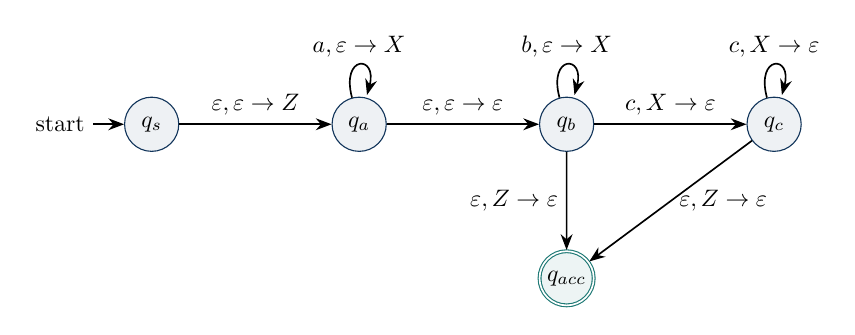
\begin{tikzpicture}[node distance=2.25cm,auto,scale=0.86,transform shape]
    \node[pda,initial] (s) {$q_s$};
    \node[pda,right=of s] (a) {$q_a$};
    \node[pda,right=of a] (b) {$q_b$};
    \node[pda,right=of b] (c) {$q_c$};
    \node[accept,below=1.45cm of b] (acc) {$q_{acc}$};

    \path
    (s) edge node {$\eps,\eps\to Z$} (a)
    (a) edge[loop above] node {$a,\eps\to X$} (a)
    (a) edge node {$\eps,\eps\to\eps$} (b)
    (b) edge[loop above] node {$b,\eps\to X$} (b)
    (b) edge node {$c,X\to\eps$} (c)
    (c) edge[loop above] node {$c,X\to\eps$} (c)
    (b) edge node[left] {$\eps,Z\to\eps$} (acc)
    (c) edge node[right] {$\eps,Z\to\eps$} (acc);
\end{tikzpicture}
\end{columns}
\end{frame}

% -------------------------------------------------
\begin{frame}{Example 10 Worked Trace}
\small
For input \(aabccc\):
\[
(q_a,aabccc,Z)
\turn(q_a,abccc,XZ)
\turn(q_a,bccc,XXZ)
\turn(q_b,bccc,XXZ)
\turn(q_b,ccc,XXXZ)
\turn(q_c,cc,XXZ)
\turn(q_c,c,XZ)
\turn(q_c,\eps,Z)
\turn(q_{acc},\eps,\eps).
\]

\begin{exampleblock}{Correctness}
The stack counts the total number of symbols in the \(a\)-block and \(b\)-block.  The final \(c\)-block must remove exactly that many markers.
\end{exampleblock}
\end{frame}

% -------------------------------------------------
\begin{frame}{Summary of the Ten PDA Patterns}
\small
\centering
\renewcommand{\arraystretch}{1.22}
\begin{tabular}{p{0.29\textwidth}p{0.58\textwidth}}
\toprule
\textbf{Language type} & \textbf{Stack role}\\
\midrule
\(a^n b^{2n}\), \(a^i b^j, i\le j\) & counter with slightly modified popping rule\\
\(a^i b^j c^k, i=k\), \(a^i b^j c^{i+j}\) & ignore irrelevant block, match total count\\
\(w\#w^R\), palindromes & store symbols and compare in reverse order\\
Balanced parentheses & store unmatched opening symbols\\
\(\#_0=\#_1\) & store current imbalance\\
\(i=j\) or \(j=k\) & nondeterministically choose a branch\\
\(a^n b^m c^m d^n\) & exploit nested LIFO structure\\
\bottomrule
\end{tabular}
\end{frame}


% -------------------------------------------------

\section{Practice and Recap}

% -------------------------------------------------
\begin{frame}{In-Class Design Problems}
Describe the stack strategy before drawing any states.

\begin{enumerate}
    \item $L_1=\lang{a^nb^{2n}\mid n\ge0}$
    \item $L_2=\lang{0^i1^j\mid i\le j}$
    \item $L_3=\lang{w\#w^R\mid w\in\{a,b\}^{*}}$
    \item $L_4=\lang{0^i1^j2^k\mid i=k}$
    \item $L_5=\lang{w\in\{0,1\}^{*}\mid w=w^R}$
\end{enumerate}

\vspace{0.7em}
For each language, identify whether nondeterminism is genuinely useful.
\end{frame}

% -------------------------------------------------
\begin{frame}{Quick Concept Check}
\begin{enumerate}
    \item Why does $\delta$ return a set of possible moves?
    \item What does the label $1,0\to\eps$ mean?
    \item Can a PDA accept with a nonempty stack under final-state acceptance?
    \item Why does $\{ww^R\}$ need a guessed midpoint but $\{w\#w^R\}$ does not?
    \item Why is consuming the entire input part of acceptance?
\end{enumerate}
\end{frame}

% -------------------------------------------------
\begin{frame}{Today’s Big Picture}
\begin{center}
\Large
\textbf{PDA = finite-state control + one unbounded LIFO stack}
\end{center}

\vspace{1em}
\begin{columns}[T,onlytextwidth]
\column{0.31\textwidth}
\begin{block}{Store}
Push information from an earlier input region.
\end{block}

\column{0.31\textwidth}
\begin{exampleblock}{Compare}
Pop to match counts or reverse-order symbols.
\end{exampleblock}

\column{0.31\textwidth}
\begin{alertblock}{Guess}
Use nondeterminism when the correct phase boundary is hidden.
\end{alertblock}
\end{columns}
\end{frame}

% -------------------------------------------------
\begin{frame}{Next Lecture}
We will develop PDA construction more systematically and connect pushdown automata with grammars.

\vspace{0.8em}
\begin{itemize}
    \item richer PDA examples;
    \item acceptance by final state versus empty stack;
    \item context-free grammars;
    \item the equivalence between CFGs and PDAs.
\end{itemize}

\vfill
\centering
\Large A stack recognizes structure that finite memory cannot.
\end{frame}

\end{document}
